\begin{figure}[!ht]
  \centering
  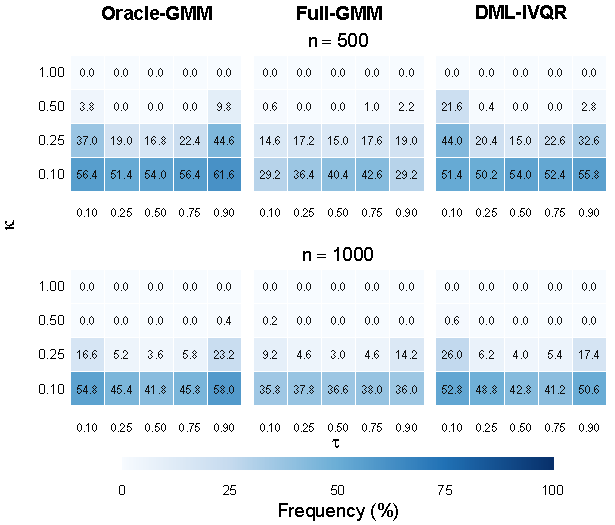
\includegraphics[width=0.72\textwidth]{figures/generated/full_domain_acceptance_heatmap.pdf}
  \caption{Full-domain grid acceptance frequencies.}
  \label{fig:appendix_full_domain_acceptance}
  \begin{figurenotes}
    Each cell reports the percentage of 500 complete replications accepting all 41 evaluated grid points in $A_0=[-1,3]$, with step size $h=0.1$. Panel columns identify estimators; panel rows show $n=500$ and $n=1000$. Within each panel, columns show quantiles $\tau$ and rows show relevance $\kappa$, declining from 1.00 to 0.10. Darker shading on the shared 0--100\% scale means more frequent full-domain grid acceptance. This event neither denotes acceptance of the entire real line nor establishes an unbounded unrestricted confidence region.
  \end{figurenotes}
\end{figure}
